\chapter{Analysis and Results}
\label{chap:eval}

\section{Introduction}

This chapter outlines the study analysis and results, which aim at identifying how machine learning
models might be used to predict the post-harvest loss (PHL) risk of smallholder agribusinesses in
Nigeria. Based on the Nigeria General Household Survey (GHS-Panel Wave~5, 2023--2024)~\cite{ghspanel2024nigeria},
the researchers estimate the behavior of post-harvest losses and determine the predictive power of
the Logistic Regression, Decision Tree, and Random Forest models. The chapter covers exploratory
data analysis, model evaluation, and important insights per the research questions.


\section{Dataset Overview and Descriptive Analysis}

This data consists of household-level agricultural data with variables such as the type of crop,
storage methods, location, and the reported causes of post-harvest losses. After processing, the
data was cleaned, missing values were imputed, and categorical values were encoded to facilitate
analysis.

\begin{figure}[htbp]
    \centering
    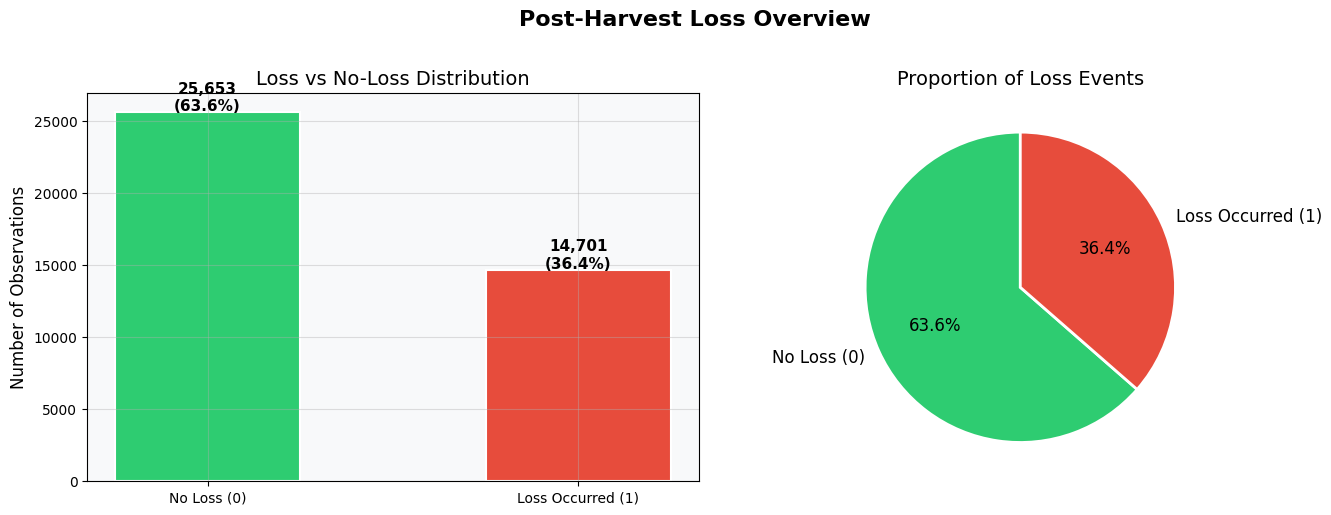
\includegraphics[width=0.85\textwidth]{attachments/figures/image1}
    \caption{Post-Harvest Loss Overview}
    \label{fig:phl-overview}
\end{figure}

Figure~\ref{fig:phl-overview} shows the total distribution of occurrences of post-harvest losses.
The findings show that post-harvest losses were observed in some 36.4 per cent of observations.
This indicates that despite the fact that some reporting areas experience more losses than others, a
significant share of smallholder farmers is affected. The evident data imbalance further defends
the implementation of extra evaluation measures such as precision and recall, rather than relying
on accuracy alone.

\begin{figure}[htbp]
    \centering
    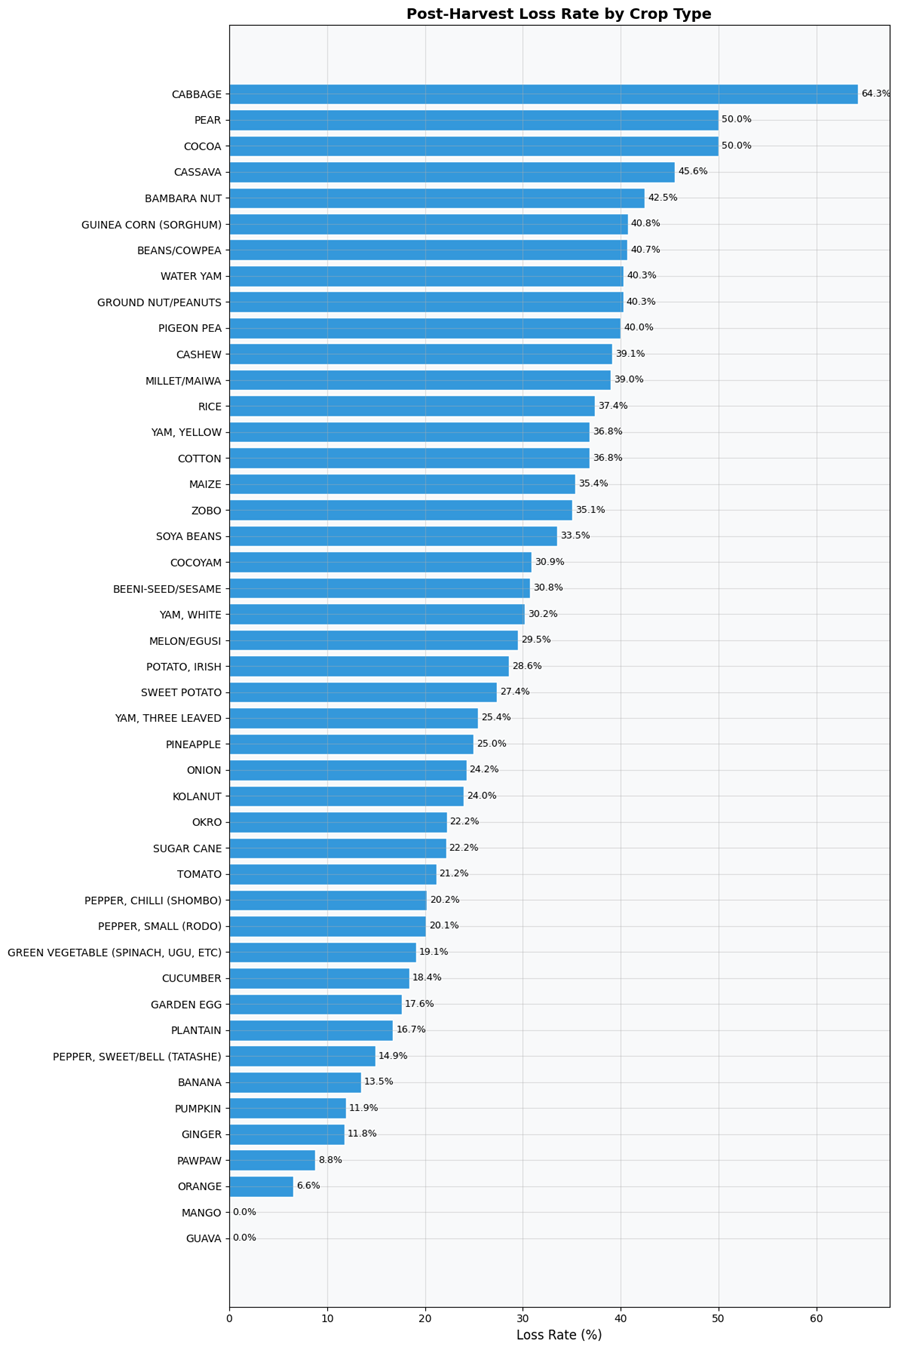
\includegraphics[width=0.75\textwidth]{attachments/figures/image2}
    \caption{Post-Harvest Loss Rates by Crop Type}
    \label{fig:phl-crop}
\end{figure}

Figure~\ref{fig:phl-crop} shows how post-harvest loss rates vary with crop type. There are crops
which have very high rates of loss, like cabbage (more than 60 per cent), while other crops like
orange and pawpaw show much lower loss rates. This difference is based on disparities in
perishability, handling needs, and storage sensitivity. The results support the validity of
post-harvest loss risk being sensitive to the type of crop, which directly answers Research
Question~1.

\begin{figure}[htbp]
    \centering
    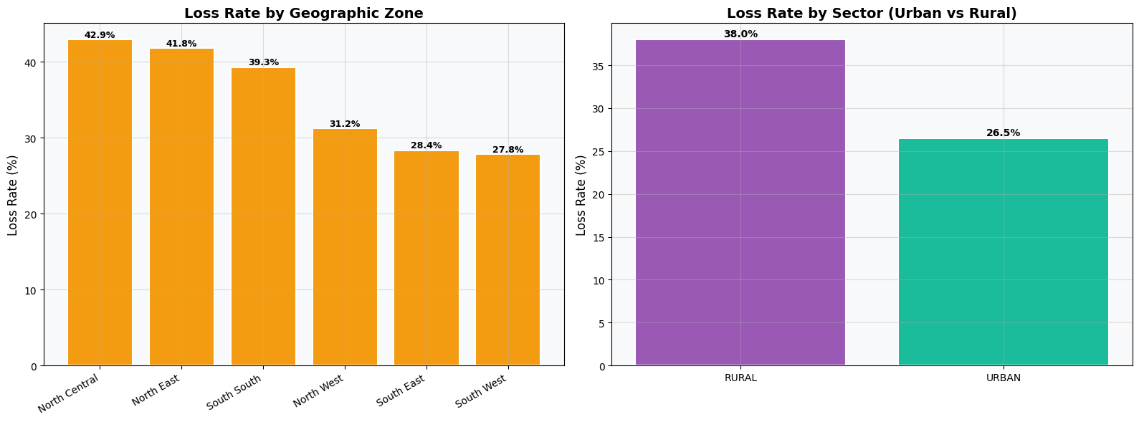
\includegraphics[width=0.75\textwidth]{attachments/figures/image3}
    \caption{Post-Harvest Loss by Geographic Zone and Sector}
    \label{fig:phl-geo}
\end{figure}

The rates of losses in each geographic region and in rural and urban spheres are shown in
Figure~\ref{fig:phl-geo}. The findings indicate a tendency for greater losses in the north than
in the south. Furthermore, the rates of loss in rural areas are significantly higher (approximately
38 per cent) than in urban areas (approximately 26 per cent). This gives a hint that
infrastructural constraints such as storage and mode of transportation have a great impact on the
extent of post-harvest losses.

\begin{figure}[htbp]
    \centering
    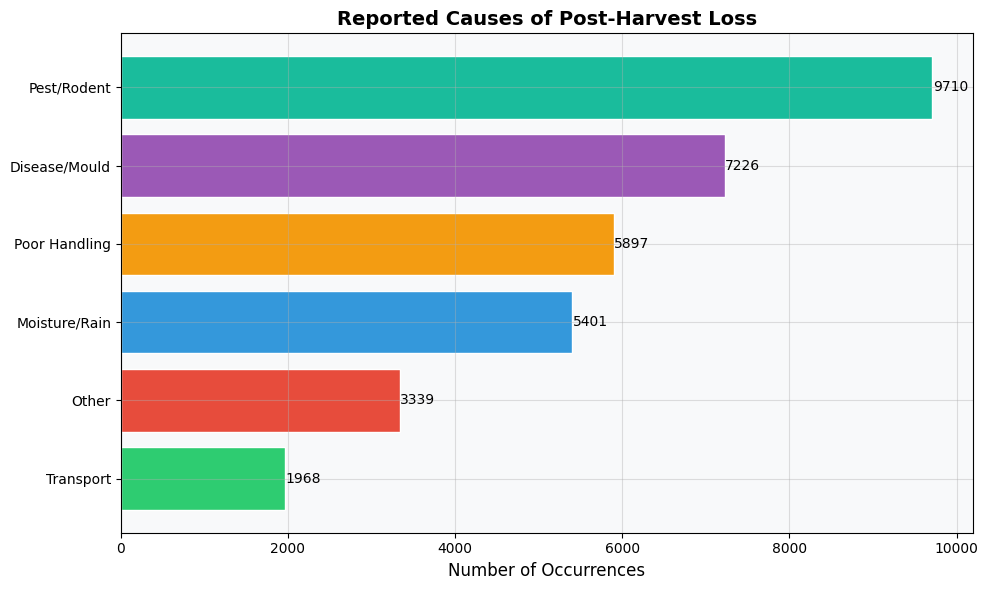
\includegraphics[width=0.65\textwidth]{attachments/figures/image4}
    \caption{Reported Causes of Post-Harvest Loss}
    \label{fig:phl-causes}
\end{figure}

Reported causes of post-harvest losses are shown in Figure~\ref{fig:phl-causes}. The most common
cause is pest and rodent infestation, followed by disease or mold and poor handling. Environmental
conditions such as moisture and rainfall also play a role. These results point to the idea that
biological and operational factors comprise the major causes of loss and therefore show the areas
most susceptible to specific interventions.

\begin{figure}[htbp]
    \centering
    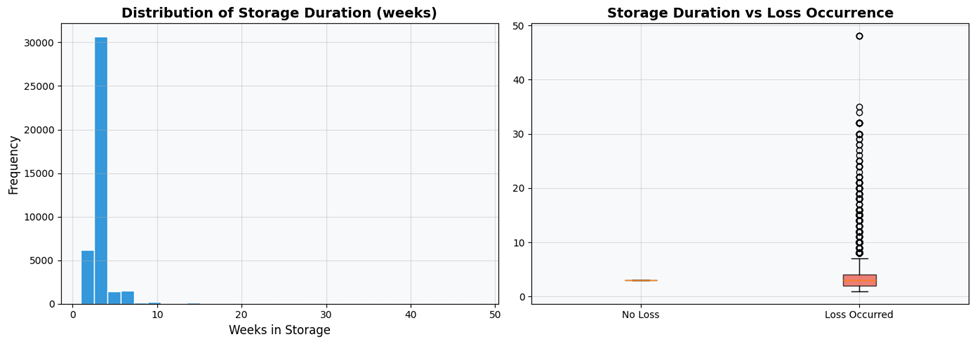
\includegraphics[width=0.75\textwidth]{attachments/figures/image5}
    \caption{Storage Duration and Loss Occurrence}
    \label{fig:phl-duration}
\end{figure}

The dependence between storage period and post-harvest loss is presented in
Figure~\ref{fig:phl-duration}. Although the majority of storage times are of rather short
character, the findings show that the longer the storage time, the higher the probability of loss.
This implies that prolonged storage without proper preservation methods increases the chances of
spoilage, underscoring the importance of proper storage management.

\begin{figure}[htbp]
    \centering
    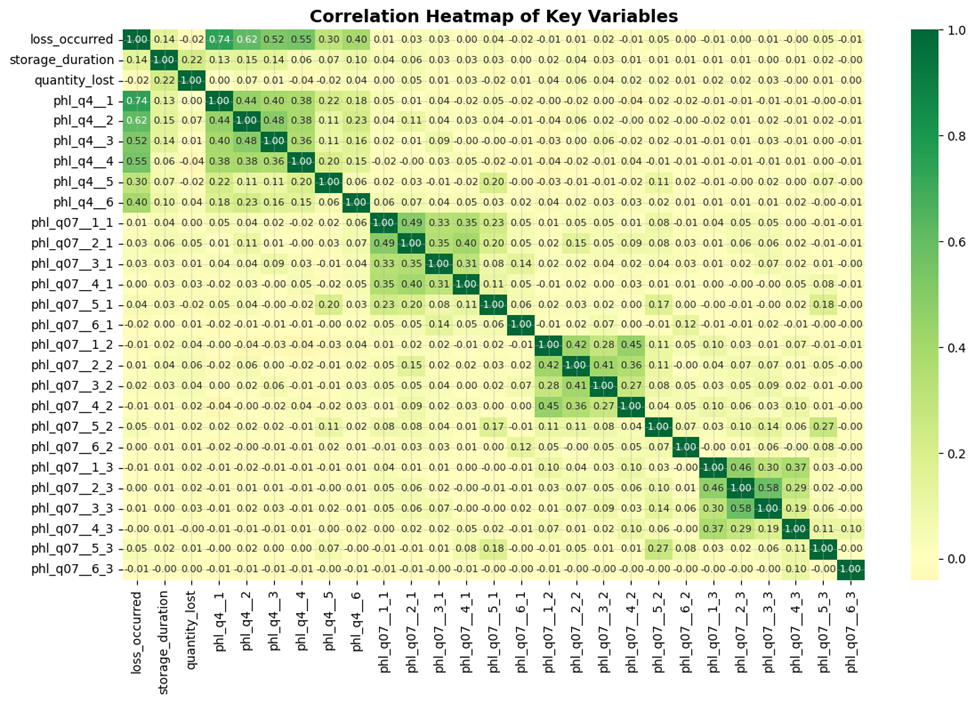
\includegraphics[width=0.75\textwidth]{attachments/figures/image6}
    \caption{Correlation Heatmap of Key Variables}
    \label{fig:phl-heatmap}
\end{figure}

The correlation between the key variables is shown in Figure~\ref{fig:phl-heatmap}. Moderate
positive relationships are observed between storage time, amount lost, and loss occurrence. Despite
the weak correlation of most variables, this can be expected given the complicated nature of
agricultural systems. The heatmap gives insight into variable relationships and aids in the
selection of features for predictive modelling.


\section{Model Performance Evaluation}

Three machine learning models were assessed: Logistic Regression, Decision Tree, and Random Forest.
They were divided into training and testing sets, and the results of model performance were
evaluated in the form of accuracy, precision, recall, F1-score, and AUC-ROC.

\begin{table}[htbp]
    \centering
    \caption{Model Performance Comparison}
    \label{tab:model-perf}
    \begin{tabular}{lccccc}
        \toprule
        \textbf{Model} & \textbf{Accuracy} & \textbf{Precision} & \textbf{Recall} & \textbf{F1-Score} & \textbf{AUC-ROC} \\
        \midrule
        Logistic Regression & 0.9742 & 1.0000 & 0.9293 & 0.9633 & 0.9715 \\
        Decision Tree       & 0.9905 & 1.0000 & 0.9738 & 0.9867 & 0.9920 \\
        Random Forest       & 0.9905 & 1.0000 & 0.9738 & 0.9867 & 0.9938 \\
        \bottomrule
    \end{tabular}
\end{table}

The findings in Table~\ref{tab:model-perf} show that both the Decision Tree and the Random Forest
models reached a high level of performance, though the Random Forest achieved a higher AUC-ROC.
Logistic Regression also showed good effectiveness but with lower recall, implying it was less
sensitive to loss cases. These results prove that machine learning models may correctly predict the
risk of post-harvest losses, responding to Research Question~2.

\begin{figure}[htbp]
    \centering
    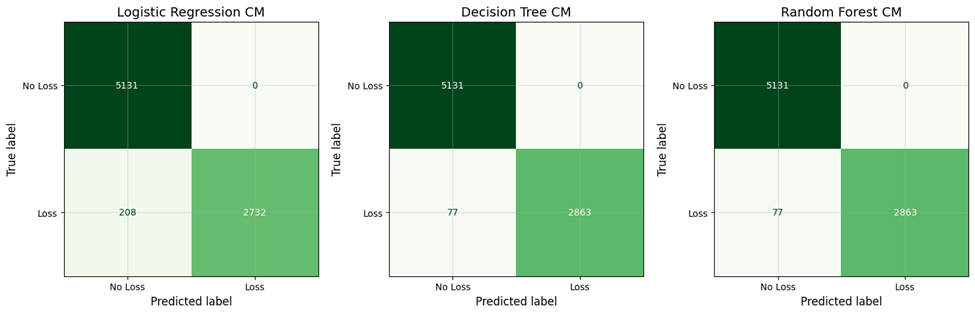
\includegraphics[width=0.80\textwidth]{attachments/figures/image7}
    \caption{Confusion Matrices for Machine Learning Models}
    \label{fig:conf-matrix}
\end{figure}

The confusion matrices are shown in Figure~\ref{fig:conf-matrix}. Random Forest had the least
number of misclassifications, confirming it as the strongest predictive model. The false negatives
were greater in Logistic Regression, meaning it is strained when complex correlations are present.
These findings also confirm the usefulness of ensemble methods.


\section{Feature Importance Analysis}

\begin{figure}[htbp]
    \centering
    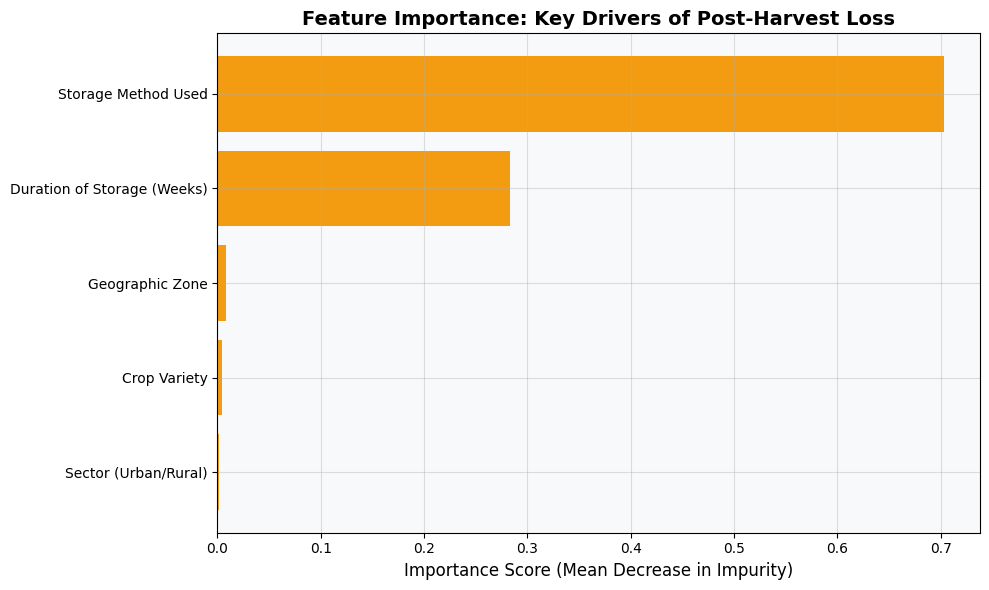
\includegraphics[width=0.60\textwidth]{attachments/figures/image8}
    \caption{Feature Importance from Random Forest Model}
    \label{fig:feat-importance}
\end{figure}

Figure~\ref{fig:feat-importance} demonstrates how features are important in predicting
post-harvest loss. Storage method becomes the most determining variable, with storage duration
coming next. Other variables, including geographic zone and crop type, are relatively less
important. These results underline the significance of storage practice on loss risk and provide
actionable guidance on how companies can minimise losses.

\begin{figure}[htbp]
    \centering
    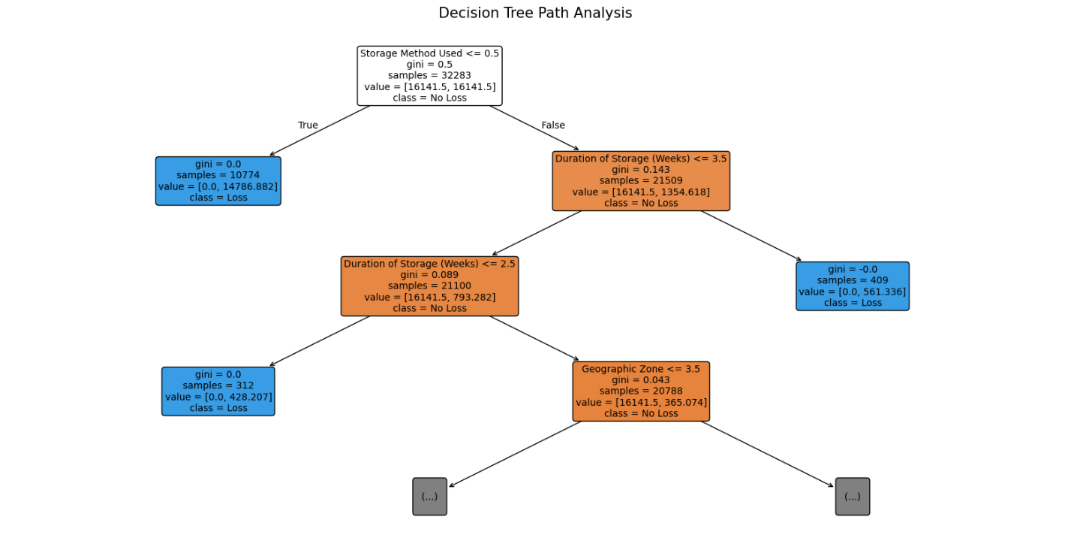
\includegraphics[width=0.75\textwidth]{attachments/figures/image9}
    \caption{Decision Tree Path Analysis}
    \label{fig:dt-path}
\end{figure}

Figure~\ref{fig:dt-path} shows the structure of the Decision Tree model. One of the key decision
points identified in the model is storage method and storage duration, pointing to their
significance in predicting outcomes. The uncovered tree may offer interpretable decision rules that
can inform useful agrobusiness decisions, responding to Research Question~3.


\section{Key Findings}

The analysis yields a number of significant findings:

\begin{itemize}
    \item A large number of smallholder farmers are impacted by post-harvest losses, with
          approximately 36.4 per cent of observations recording a loss event.
    \item The loss rates differ significantly depending on the type of crop, with perishable
          crops registering the highest loss rates.
    \item Distribution of losses depends on geographic and infrastructural location, with rural
          places being more affected than urban areas.
    \item The most significant predictors of post-harvest loss are storage method and storage
          duration.
    \item Among the models evaluated, Random Forest showed the best predictive performance as
          measured by AUC-ROC.
\end{itemize}


% =============================================================
\chapter{Discussion}
\label{chap:discuss}
% =============================================================

\section{Introduction}

This chapter critically reflects on the findings reported in Chapter~\ref{chap:eval} within the
larger academic and practical framework of post-harvest loss management and machine learning in the
agricultural industry. The research questions are used to organize the discussion by correlating
empirical findings with the literature. It assesses the potential implications of the findings on
theory and practice, the limitations of the study, and future research possibilities.


\section{Discussion of Key Findings}

\subsection{Factors Influencing Post-Harvest Loss (RQ1)}

This research has shown that the most influential factors determining post-harvest loss are the
storage method, storage period, type of crop, and geographic location. Of these, storage-related
variables proved to be most influential, as seen in the feature importance analysis and the decision
tree structure.

This conclusion is very much in agreement with the literature. According to
\cite{rajapaksha2021reducing}, poor storage systems contribute more significantly to post-harvest
losses in developing nations, especially for perishable goods. In the same vein,
\cite{wakene2024comprehensive} point out that inappropriate storage leads to faster spoilage, as is
the case with most environmentally sensitive crops like tomatoes. These conclusions are supported in
the present study, which proves in a quantitative way that storage method is the most significant
predictor of loss risk.

This argument is also supported by the significance of storage period. According to the results,
the longer the storage, the higher the risk of losses, which is also consistent with the work of
\cite{ukwuaba2024mitigating}, who show that prolonged storage is one of the main factors leading to
losses in cucumber production. This implies that the quality of storage and the time goods are kept
should both be managed to reduce spoilage.

Type of crop was also revealed to be a major aspect, with highly perishable crops like cabbage
showing greater levels of losses. This observation aligns with \cite{oluoch2024causes}, who state
that leafy vegetables are especially susceptible to post-harvest degradation because of their high
moisture level and fragility during handling. The difference in loss levels across different crops
underscores the necessity to focus on crop-specific post-harvest methods.

Infrastructure differences are depicted in geographic variations in losses. The findings reveal a
stronger loss rate in the north and rural regions, consistent with \cite{pluato2024impact}, who
report post-harvest losses as being more severe in locations with low infrastructure, poor storage
facilities, and inadequate transportation networks. These results highlight the significance of
socio-economic and environmental circumstances in determining post-harvest outcomes.

The findings substantiate the assumption that post-harvest losses are the result of intertwined
operational, environmental, and infrastructural factors. This reinforces the conceptual framework
adopted in the literature review and emphasises the need to use integrated methods to reduce losses.

\subsection{Predictive Accuracy of Machine Learning Models (RQ2)}

The paper shows that structured agricultural data using simple machine learning models can
successfully predict the risk of post-harvest losses. Random Forest was the top model among those
tested, with Decision Tree coming in closely after, while Logistic Regression showed lower recall.

These results align with current studies in the field of machine learning in agriculture.
\cite{jabed2024crop} note that ensemble techniques, including Random Forest, are especially useful
in adopting difficult, non-linear associations in farm-based data. This claim is supported by the
better outcome of the Random Forest in the present study, suggesting that post-harvest loss is
determined by the combination of many interacting factors, which cannot be best explained by linear
techniques.

In the same way, \cite{meghraoui2024applied} focus on the fact that tree-based models are very
appropriate for agricultural prediction tasks as they can process heterogeneous data and capture
non-linear interactions. Their high results for the Decision Tree and Random Forest models in this
research affirm their appropriateness in predicting post-harvest loss risk.

The lower performance of Logistic Regression indicates the weakness of the linear methodology in
complicated agricultural systems. Although logistic regression is interpretable, it can simplify
variable relationships and hence lower predictive accuracy. This observation supports the essence
of using models appropriate to the type of data.

The high accuracy achieved in this research can indicate that there exist high-quality predictor
features, represented as storage method and loss-related variables. Although this improves model
performance, concerns about data quality and overfitting are also raised. However, the validity
of the results is enhanced by the use of several evaluation metrics and model comparison. In
general, the results show that simple and understandable machine learning models can be highly
predictive, even on small datasets.

\subsection{Application of Predictions in Decision-Making (RQ3)}

The important contribution that this study makes is to show that machine learning predictions can
be useful in helping to make practical decisions in agribusiness. The findings indicate that
predictive models have the ability to determine high-risk situations, which are dependent on storage
approach and time, and therefore allow farmers to make advance actions.

This is in line with the concept of decision support systems (DSS) in the agricultural sector.
\cite{duan2021multicriteria} believe that DSS has the potential to increase agro productivity
because it can help convert information into action. The given research builds upon that idea by
demonstrating how machine learning models can serve as the core of such systems, giving risk
forecasts that are used in decision-making.

The interpretability of Decision Trees adds further practical value. The model's rule-based format
enables farmers and stakeholders to understand the circumstances under which a loss is probable.
For example, storage duration thresholds revealed in the model can be applied in deciding optimum
storage times. This proves how predictive models can be converted into rules that can be easily
implemented in practice.

In addition, storage practices are identified as key factors for intervention. The risks of losses
can be significantly minimized by improving storage methods or decreasing storage time. These
lessons can be especially useful to smallholder farmers who require economical and feasible
solutions. The output of such decision support systems is however determined by their access and
use. According to \cite{duan2021multicriteria}, most existing systems are excessively complicated
in the context of the smallholder. This research addresses this gap by concentrating on simple and
interpretable models which can be applied using easily accessible data.


\section{Theoretical Implications}

This research contributes to the growing literature on machine learning in agriculture by
demonstrating its applicability to post-harvest loss prediction. The study shows that machine
learning can be used to address the problem of post-harvest management~\cite{jabed2024crop,meghraoui2024applied}.
The results also support the criticality of incorporating data-driven strategies with conventional
agricultural wisdom. The study offers a more systematic analysis of what drives loss after harvest
by determining the strength of key drivers of losses. This helps in the creation of better
theoretical models of agricultural systems.


\section{Practical Implications}

The applications of this study are highly practical. For smallholder farmers, the findings provide
clear guidelines on how to reduce post-harvest losses. Better storage, shorter storage durations,
and more efficient handling practices can play a great role in minimizing losses.

For policymakers, the findings demonstrate the importance of investment in storage facilities and
training programmes. The geographic variations in loss rates can be reduced by addressing
infrastructural differences between areas.

For agribusiness stakeholders, the research proves the importance of data-driven decision-making.
Simple machine learning models can be implemented to improve supply chain efficiency and minimize
losses along the way.


\section{Limitations of the Study}

Although it contributed within its confines, there are a few limitations of this study. Since it uses a dataset covering one country, the findings might be of limited generalisability to other
settings. Also, the data is cross-sectional, which makes it impossible to analyze temporal changes in post-harvest losses. The high performance of the models can indicate the existence of strong
predictive features, which increases the chances of overfitting. Moreover, the research centers on few variables, and additional factors including market forces and climate change may further enhance
predictive ability.


\section{Future Research Directions}

Future study may build on this work by including bigger and more varied datasets, such as
multi-country data. There would be an opportunity to include environmental variables (e.g.\
temperature, precipitation) that would benefit model performance. Besides, further examination of
more sophisticated machine learning algorithms such as deep learning might yield more information,
but should be weighed against the requirement of interpretability. The development and testing of
real-time decision support systems would also help to close the gap between research and practice.
